\documentclass[tikz,border=2pt]{standalone}
\usepackage{amsmath}
\usepackage{pgfplots}
\pgfplotsset{compat=1.18}
\usetikzlibrary{arrows.meta}
\begin{document}
% Example 7.1: max 3x_1+5x_2, x_1<=4, 2x_2<=12, 3x_1+2x_2<=b_3. As b_3 runs over [12,24] (delta in [-6,6])
% the line 3x_1+2x_2=b_3 shifts in parallel and the optimal corner slides along 2x_2=12 from (0,6) to (4,6).
% The scale below the x_1-axis is b_3=3x_1, the x_1-intercept of the moving line.
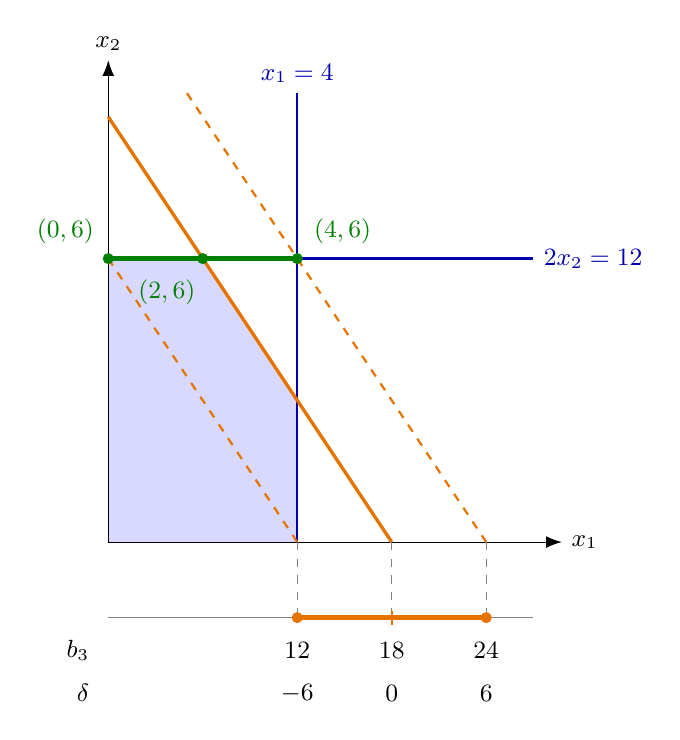
\begin{tikzpicture}[font=\small, >={Latex[length=2mm]}, x=0.6cm, y=0.6cm]
  % feasible region for b_3=18
  \fill[blue!15] (0,0) -- (4,0) -- (4,3) -- (2,6) -- (0,6) -- cycle;
  % axes
  \draw[->] (0,0) -- (9.6,0) node[right] {$x_1$};
  \draw[->] (0,0) -- (0,10.2) node[above] {$x_2$};
  % fixed constraints
  \draw[blue!70!black, thick] (4,0) -- (4,9.5) node[above] {$x_1=4$};
  \draw[blue!70!black, thick] (0,6) -- (9,6) node[right] {$2x_2=12$};
  % the moving third constraint 3x_1+2x_2=b_3
  \draw[orange!90!black, thick, dashed] (0,6) -- (4,0);
  \draw[orange!90!black, very thick] (0,9) -- (6,0);
  \draw[orange!90!black, thick, dashed] (5/3,9.5) -- (8,0);
  % path of the optimal corner
  \draw[green!50!black, line width=2pt] (0,6) -- (4,6);
  \fill[green!50!black] (0,6) circle (2pt) (2,6) circle (2pt) (4,6) circle (2pt);
  \node[green!50!black, anchor=south east] at (-0.1,6.1) {$(0,6)$};
  \node[green!50!black, anchor=north east] at (2.05,5.75) {$(2,6)$};
  \node[green!50!black, anchor=south west] at (4.15,6.1) {$(4,6)$};
  % scale for b_3 = 3 x_1 (x_1-intercept of the moving line)
  \foreach \x in {4,6,8} \draw[gray, thin, dashed] (\x,0) -- (\x,-1.6);
  \draw[gray] (0,-1.6) -- (9,-1.6);
  \draw[orange!90!black, line width=2pt] (4,-1.6) -- (8,-1.6);
  \fill[orange!90!black] (4,-1.6) circle (2pt) (8,-1.6) circle (2pt);
  \draw[orange!90!black, thick] (6,-1.75) -- (6,-1.45);
  \node[anchor=east] at (-0.2,-2.3) {$b_3$};
  \node[anchor=east] at (-0.2,-3.2) {$\delta$};
  \node at (4,-2.3) {$12$};
  \node at (6,-2.3) {$18$};
  \node at (8,-2.3) {$24$};
  \node at (4,-3.2) {$-6$};
  \node at (6,-3.2) {$0$};
  \node at (8,-3.2) {$6$};
\end{tikzpicture}
\end{document}
